%Preamble
    \documentclass[12pt]{article}
  
    \usepackage[paperheight=150mm,paperwidth=200mm,hmargin=30mm,bmargin=20mm]{geometry}
    \bibliographystyle{astron} 
    \usepackage{natbib}
    \usepackage{amssymb}
    \usepackage{amsmath}
    \usepackage[titletoc]{appendix}
    \usepackage{mdwlist}
    \usepackage{changepage}
    \usepackage{booktabs}
    \usepackage{float}
    \usepackage{graphicx}
    \usepackage{leftidx}
    \usepackage{multicol}
    \usepackage{hyperref}
    \usepackage{xcolor}
    \usepackage{setspace}
    \setlength{\parskip}{0.5\baselineskip}
    \setlength{\parindent}{0pt}
    \linespread{1.2}
    \definecolor{DarkBlue}{RGB}{43,43,222}%Define a Color
    \definecolor{MyGrey}{RGB}{43,43,93}
    \hypersetup{
                colorlinks,
                breaklinks,
                urlcolor=DarkBlue,
                linkcolor=MyGrey,
                pdftitle={A Slide Template},
                pdfauthor={Fanyi Meng},
                citecolor=MyGrey
                }

    \newcommand{\dd}{{\rm d}}
    \newcommand{\coa}{$\rm ^{12}CO$ }
    \newcommand{\cob}{$\rm ^{13}CO$ }
    \newcommand{\coc}{$\rm C^{18}O$ }
    \newcommand{\coaa}{$\rm^{12}CO(1-0)$ }
    \newcommand{\cobb}{$\rm^{13}CO(1-0)$ }
    \newcommand{\cocc}{$\rm C^{18}O(1-0)$ }
    \newcommand{\multi}{$\times$}
    \newcommand{\vlsr}{${\rm V } _{lsr}$}
    \newcommand{\kms}{$\rm km\ s^{-1}$}
    \newcommand{\ta}{$T_{\rm A}$}
    \newcommand{\texc}{$T_{\rm {ex}}$ }
    \newcommand{\taub}{$\tau _{13}$}
    \newcommand{\tauc}{$\tau _{18}$}
    \newcommand{\tcoa}{$T_{12}$}
    \newcommand{\tcob}{$T_{13}$}
    \newcommand{\tcoc}{$T_{18}$}
    \newcommand{\nb}{$N_{13}$\ }
    \newcommand{\nc}{$N_{18}$\ }
    \newcommand{\nhyd}{$N_{\rm H_2}$\ }
    \newcommand{\nnhyd}{$n_{\rm H_2}$\ }
    \newcommand{\pow}[1]{$\times 10^{#1}$}
    \newcommand{\epm}{$\pm$}
    \newcommand{\pcms}{$\rm cm^{-2}$}
    \newcommand{\sigmath}{$\sigma _{Therm}$\ }
    \newcommand{\sigmant}{$\sigma _{NT}$\ }
    \newcommand{\sigmatd}{$\sigma _{3D}$\ }
    \newcommand{\sun}{\odot}
    %%%%%%%%%%%%%%%%%%%%%%%%%%%%%%%%%%%%%%%%%%%%%%%%%%%%%%%%%%%%%%%%%%%%%%%%
    \newcommand{\jj}{{\rm j}}
    \newcommand{\uph}{$\phi$($^{\circ}$)}
    \newcommand{\apjs}{ApJS}
    \newcommand{\apjl}{ApJL}
    \newcommand{\apj}{ApJ}
    \newcommand{\aap}{A\&A}
    \newcommand{\araa}{ARA\&A}
    \newcommand{\mnras}{MNRAS}
    \newcommand{\nat}{Nature}
    \newcommand{\aj}{AJ}
    \newcommand{\arcsec}{$^{\prime\prime}$}
    \newcommand{\arcmin}{$^{\prime}$}
    \newcommand{\arcdeg}{$^{\circ}$}

    \renewcommand{\contentsname}{Outline}

    \definecolor{darkblue}{rgb}{0.2, 0.2, 0.4}
    \definecolor{darkgrey}{rgb}{0.2, 0.2, 0.2}

    \title{\textbf{Interstellar Turbulence}}
    \author{\textsc{Fanyi Meng}\\
            Supervisor: \textsc{Prof. Yuefang Wu}}

\begin{document}
\maketitle\label{sec:title}
\clearpage
\tableofcontents
\clearpage
\section{Power Sources for Interstellar Turbulence} % (fold)
\label{sec:power_sources_for_interstellar_turbulence}
\begin{itemize}
    \item Stars: protostellar winds, expanding H\textsc{ii} regions, O star and Wolf-Rayet winds, supernovae, and  combinations of these producing "\emph{superbubbles}";
    \item Galactic rotation in the shocks of spiral arms or bars, in the Balbus-Hawley instability, and in the gravitational scattering of cloud complexes at different epicyclic phases;
    \item Gaseous self-gravity through swing-amplified instabilities and cloud collapse;
    \item Kelvin-Helmholtz and other fluid instabilities;
    \item Galactic gravity during disk-halo circulation, the Parker instability, and galaxy interactions.
\end{itemize}
\clearpage
\cite{1985ApJ...294..567V} estimated that winds from massive main-sequence stars and Wolf-Rayet stars contribute comparable amounts, $1 \times 10^{-25}$ erg cm$^{-3}$ s$^{-1}$, supernovae release about twice this, and winds from low-mass stars and planetary nebulae are negligible.

\cite{2004RvMP...76..125M} found that main-sequence winds are negligible except for the highest-mass stars, in which case supernovae dominate all the stellar sources, giving $3 \times 10^{-26}$ erg cm$^{-3}$ s$^{-1}$ for the energy input, after multiplying by an efficiency factor of 0.1. \cite{2004RvMP...76..125M} also derived an average injection rate from protostellar winds equal to $2 \times 10^{-28}$ erg cm$^{-3}$ s$^{-1}$  including an efficiency factor of $\sim 0.05$.

Turbulent heating rate inside a giant molecular cloud (GMC)  $\sim 1-6 \times 10^{-27} n_H\Delta v^3 / R \rm \  erg\ cm^{-3}\ s^{-1}$ \citep{1998ApJ...508L..99S}.
% section power_sources_for_interstellar_turbulence (end)
\newpage
\section{Reynold Number} % (fold)
\label{sec:Reynold Number}
    {Cloudy objects with a hierarchy structures form in \textbf{interacting shock waves} by supersonic turbulence that is \textbf{stirred on the largest scale} by differential galactic rotation and \textbf{dissipated on small scales} by atomic viscosity} \citep{1951ApJ...114..165V}.


    \begin{equation}
        \frac{l}{\lambda} \gg 1
    \end{equation}

    $l$: the characteristic length; \\
    $\lambda$: the mean free path of the \emph{single bodies} in fluid.

    While the Reynold number in a flow with viscosity of $\mu$ is:
    \begin{align} 
        R& = \frac{\rho v l }{\mu} {,\ \rm where\ } 
        \mu = \rho v_{th} \lambda\\
        &=\frac{vl}{v_{th}\lambda}
    \end{align}

    if:
    \begin{align} 
        \frac{l}{\lambda} \gg 1 {\ \rm and\ } 
        \frac{v}{v_{th}}\gtrsim 1{,\ \rm then\ } 
        R\gg 1
    \end{align}
    Conventionally, $R\gtrsim 10^{3}$ is considered to be the condition when \textbf{turbulence} arises.
    Adopting our \emph{Planck} Cold Cores in Taurus as instances:
    \begin{align}
        \langle {v}/{v_{th}} \rangle &= 1.5\\
        \langle {l}/{\lambda} \rangle & = \frac{0.24\ {\rm pc}}{4\times10^{12}\ {\rm cm}} = 2\times10^{5}\\
        \langle R \rangle &= 3\times10^{5}
    \end{align}
    
    where:
    \begin{align}
        \lambda &  = \frac{1}{n\sigma}
    \end{align}
    \clearpage
% section Reynold Number (end)
\section{Kolmogorov's 5/3 Theory} % (fold)
Following are based on \emph{Computational Fluid Dynamics}, course material by \textsc{Andr\'{e} Bakker
}.
\label{sec:kolmogorov_s_5_3_theory}
    \subsection{Large Eddies} % (fold)
    \label{sub:eddies}
        \begin{itemize}
            \item Turbulence can be conceived consisting of \textbf{eddies}.
            \item Eddies of size $l_0$ have a characteristic velocity $u_0$ and timescale $\tau_0=l_0/u_0$.
            \item Eddy's characteristic velocity: $u_0\equiv u(l_0)\sim \sqrt{2E_k(l_0)/3}$
            \item Eddy will dissipate within time scale $\tau_0$, due to viscosity $\mu$, with dissipation rate $\varepsilon$.
        \end{itemize}

        Thus we can obtain the integral length scale $l_0$:
        \begin{equation}
            l_0 \propto \frac{k^{3/2}}{\varepsilon}
        \end{equation}
    % subsection eddies (end)
    \clearpage
    \subsection{Energy Cascade} % (fold)
    \label{sub:energy_cascade}
        \begin{itemize}
            \item Energy is transferred form larger eddies to the smaller ones inside them, resembling recursion.
            \item Such \emph{cascade} halt when the Reynold number: $R = \rho u l /\mu$ is small enough at small scales.
            \item At small scales, $E_k$ is converted to heat, which is \textbf{dissipation}.
        \end{itemize}
    In such dissipation, the energy transfer rate can be estimated as:
    \begin{equation}
        \varepsilon = \frac{\partial E_k}{\partial t} \propto \frac{u_0^2}{\tau_0}=\frac{u_0^3}{l_0}
    \end{equation}

    Such a $\varepsilon$ consists well with FD experiments and is remarkably irrelevant to fluid viscosity $\mu$. 
    % subsection energy_cascade (end)
    \clearpage
    \subsection{Kolmogorov's Hypotheses} % (fold)
    \label{sub:kolmogorov_s_hypotheses}
    \begin{itemize}
        \item At sufficiently high Reynolds numbers, the small-scale turbulent motions 
    ($l \ll l_0$) are statistically isotropic.
        \item In every turbulent flow at sufficiently high Reynolds number, the statistics of the small scale motions ($l<l_{EI}$) have a universal form that is uniquely determined by $\varepsilon$ and $\nu$. (Hereafter, we denote $\mu/\rho$ as $\nu$ for clarity.)
        \item In every turbulent flow at sufficiently high Reynolds number, the statistics of the motions of scale l in the range $l_0 \gg l \gg \eta$ have a universal form that is uniquely determined by $\varepsilon$ independent of $\nu$.
    \end{itemize}

    Adopting these hypotheses and \emph{dimensional analysis}, we can get following approximations.
    % subsection kolmogorov_s_hypotheses (end)
    \clearpage
    \subsection{Kolmogorov Scales} % (fold)
    \label{sub:kolmogorov_scales}
        If we assume that in small scale, the \textbf{sufficient small Reynold number} is 1, as we have already obtained that $\varepsilon = u^3/l$, $\nu = ul$, we can easily write following parameters as power functions of them.
        \begin{align}
            \eta &= (\nu^3/\varepsilon)^{1/4}\\
            u_{\eta} &= (\nu \varepsilon)^{1/4}\\
            \tau_{\eta} &= (\nu/\varepsilon)^{1/2}
        \end{align}
        and the ratio of them to corresponding parameters at large scales:
        \begin{align}
            \eta/l_0 &\sim R_L^{-3/4}\\
            u_{\eta}/u_0 &= R_L^{-1/4}\\
            \tau_{\eta}/\tau_0 &= R_L^{-1/2}
        \end{align}
        where $R_L\equiv {u_0 l_0}/{\nu}$
    % subsection kolmogorov_scales (end)
    \clearpage
    \subsection{Middle Scales: Inertial Subrange} % (fold)
    \label{sub:middle_scales_inertial_subrange}
    Inertial subrange are of eddy at middle scales that only with energy transferred in and out, but not dissipated. 
    \begin{align}
        u(l)&=(\varepsilon l)^{1/3}&=u_\eta(1/\eta)^{1/3}&\sim u_0(l/l_0)^{1/3}\\
        \tau(l) &=(l^2/\varepsilon)^{1/3}&=\tau_\eta(1/\eta)^{2/3}&\sim \tau_0(l/l_0)^{2/3}
    \end{align}
    \begin{figure}[hb]
              \centering
              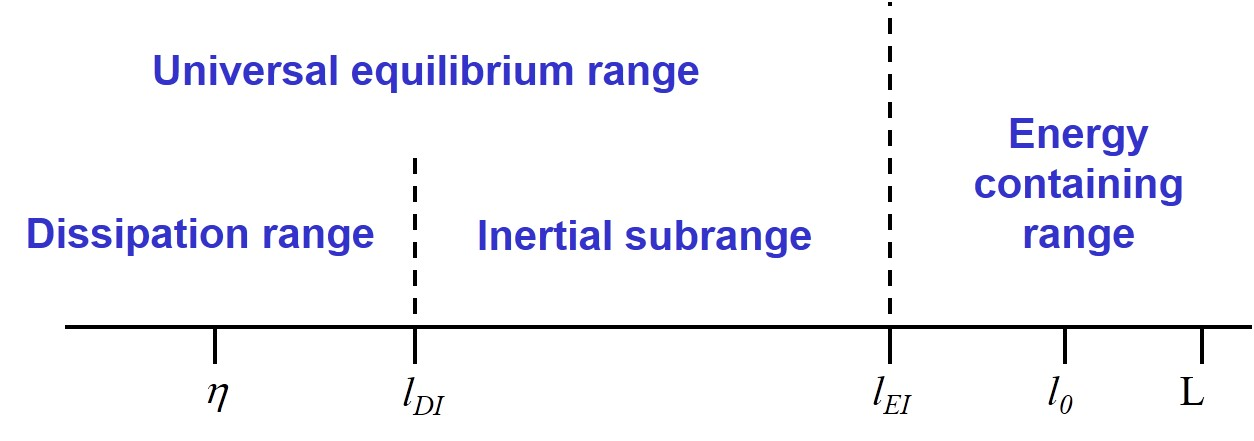
\includegraphics[totalheight=45 mm]{img/ranges.jpg}
    \end{figure}
    % subsection middle_scales_inertial_subrange (end)
    \clearpage
    \subsection{Energy spectrum} % (fold)
    \label{sub:energy_spectrum}
        The power spectrum of observable $A(r)$ is defined as:
        \begin{equation}
            P(k)  = \hat{A}(k)\hat{A}(k)^*
        \end{equation}
        where the $A(k)$ is the Fourier transformation of $A(r)$:
        \begin{equation}
            \hat{A}(k) = \int _0 ^\infty e^{ikr}A(r)\dd r
        \end{equation}

        If we consider \textbf{energy spectrum} $E(k)$ is one-dimensional and:
        \begin{equation}
            E(k)\dd k = P(\vec{k})\dd k ^D
        \end{equation}
        \clearpage

        Simply we regard the turbulent kinetic energy as: 
        \begin{equation}
            E_k = \frac{1}{2} (\overline{v_x^2}+\overline{v_y^2}+\overline{v_z^2})
        \end{equation}
        The spectrum $E(k)$ is the kinetic energy contained in eddies with wavenumber $k$:
        \begin{equation}
            E_k (k_A<k<k_B) = \int _{k_A}^{k_B} E(k) \dd k
        \end{equation}

        In Inertial Subrange, the $E(k)$ should only depends on $\varepsilon$ and $k$. We can adopt the \textbf{dimensional analysis}:
        \begin{equation}
            [E_k]  = m^2s^{-2};\ [\varepsilon] = m^2s^{-3};\ [k] = m^{-1};
        \end{equation}
        \begin{equation}
            [E(k)]=[E_k]/[k] = m^3s^{-2} = [\varepsilon^{2/3}k^{-5/3}]
        \end{equation}
        Thus:
        \begin{equation}
            E(k) \propto \varepsilon^{2/3}k^{-5/3}
        \end{equation}
        \clearpage
            \begin{figure}[hb]
              \centering
              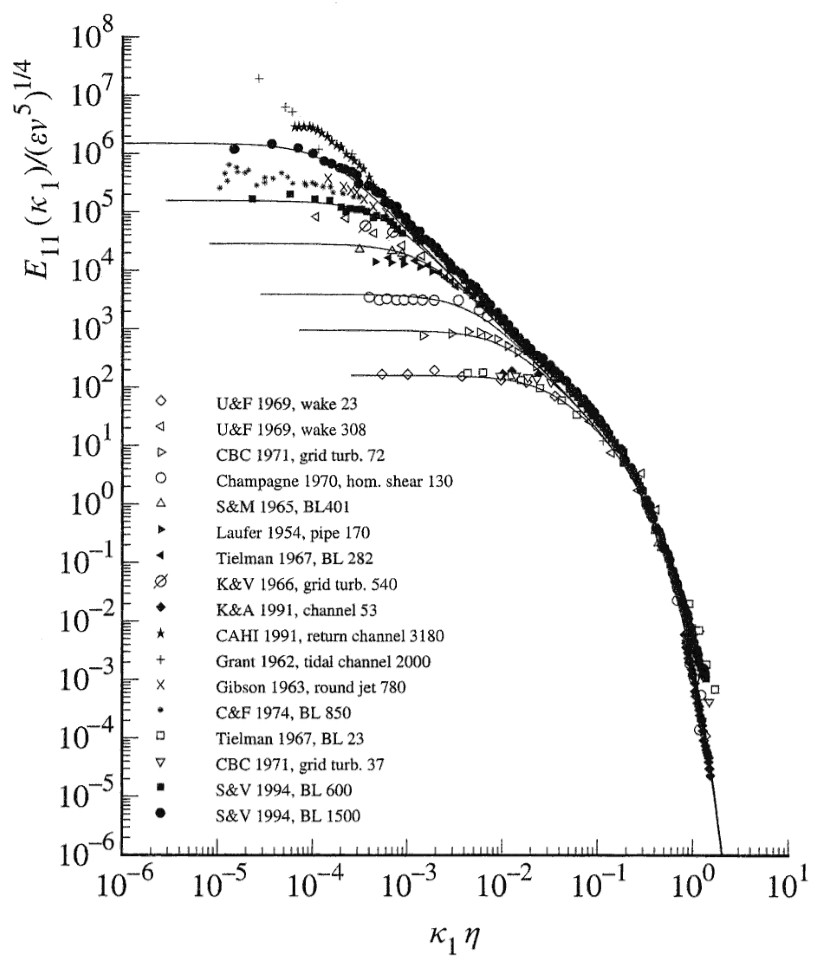
\includegraphics[totalheight=105 mm]{img/experiments.jpg}
            \end{figure}
        \clearpage
        \begin{small}
        \cite{2000ApJ...539L.133P}
        \end{small}
            \begin{figure}[hb]
              \centering
              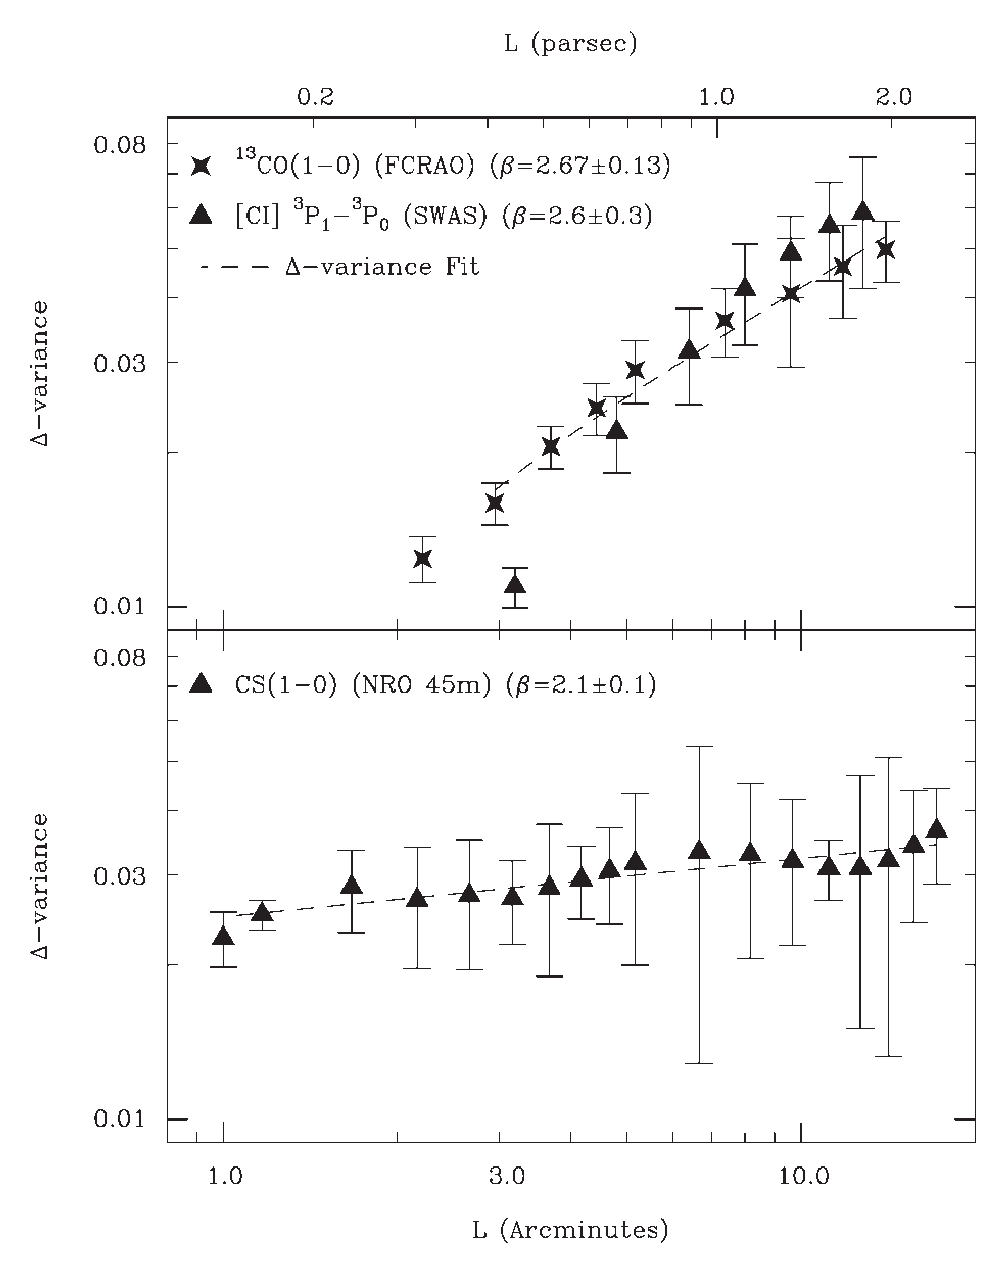
\includegraphics[totalheight=80 mm]{img/Plume2000.eps}
            \end{figure}
        \clearpage
        \begin{small}
        \cite{2001ApJ...548..749E}
        \end{small}
            \begin{figure}[hb]
              \centering
              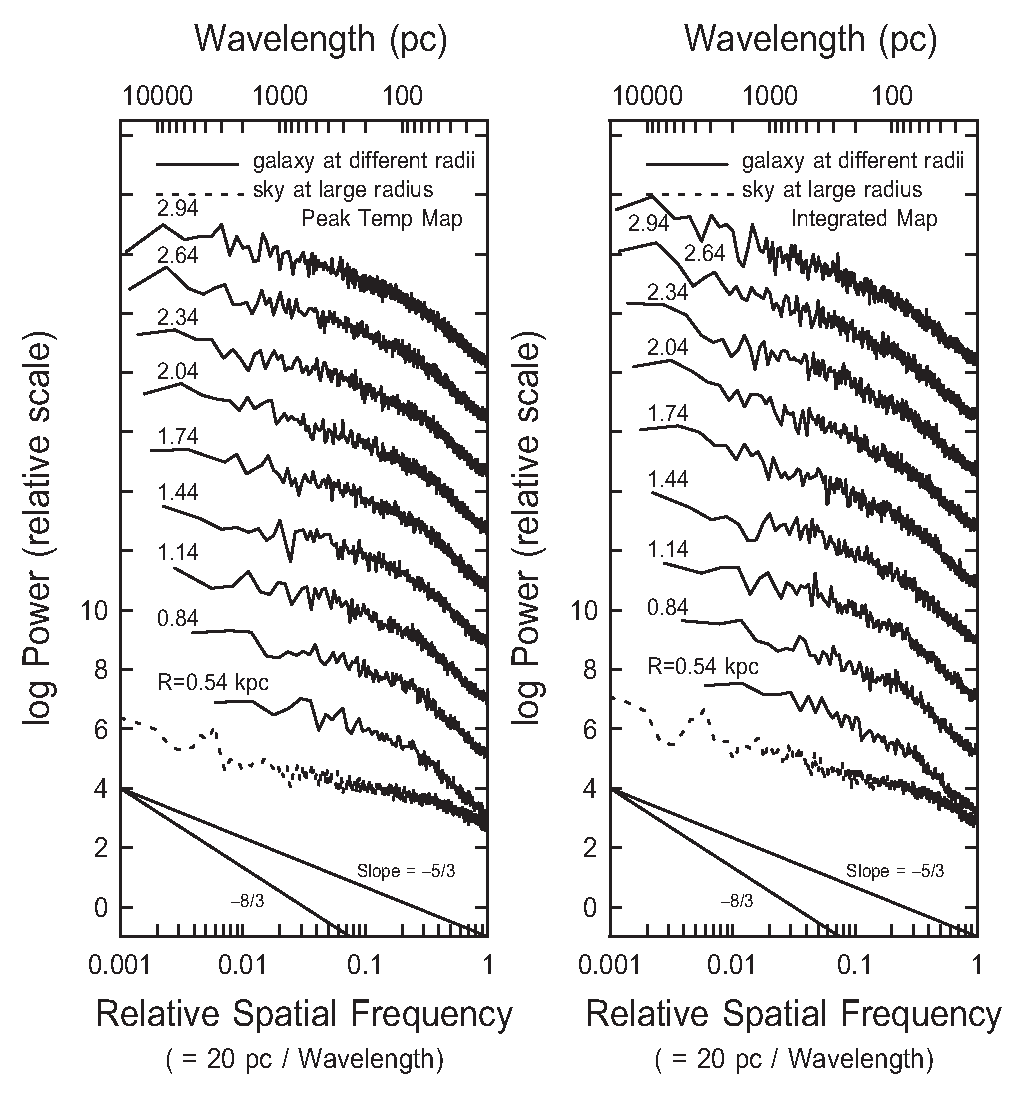
\includegraphics[totalheight=80 mm]{img/Elmegreen2001.eps}
            \end{figure}   
        \clearpage
        \begin{small}
        Southern Galactic plane H\textsc{i} survey by \cite{2001ApJ...561..264D}, region 1.
        \end{small}
            \begin{figure}[hb]
              \centering
              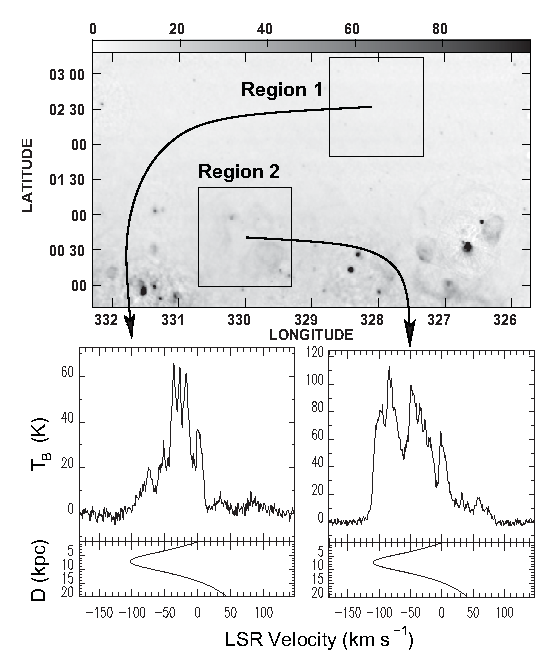
\includegraphics[totalheight=80 mm]{img/Dickey2001_regions.eps}
              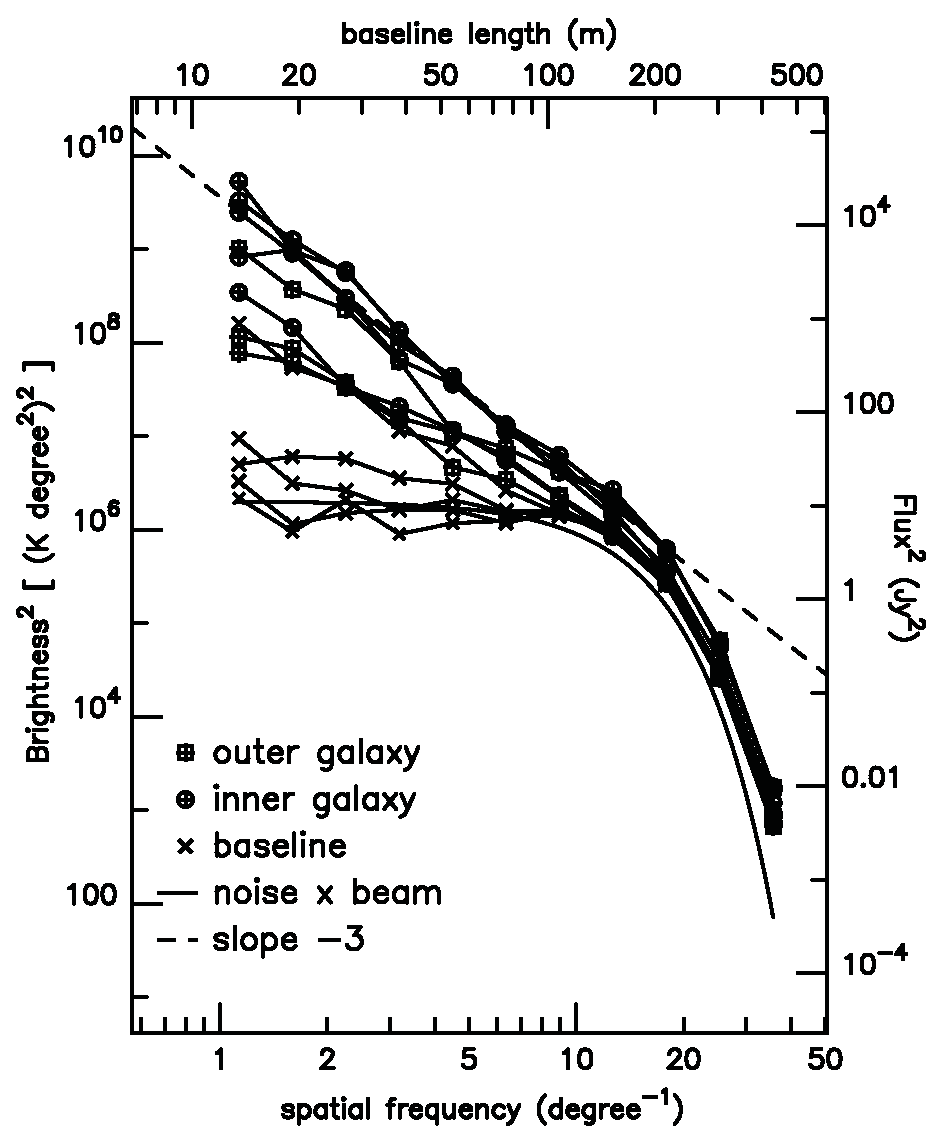
\includegraphics[totalheight=80 mm]{img/Dickey2001_region1.eps}
            \end{figure}   
        \clearpage
        \begin{small}
        Southern Galactic plane H\textsc{i} survey by \cite{2001ApJ...561..264D}, region 2.
        \end{small}
            \begin{figure}[hb]
              \centering
              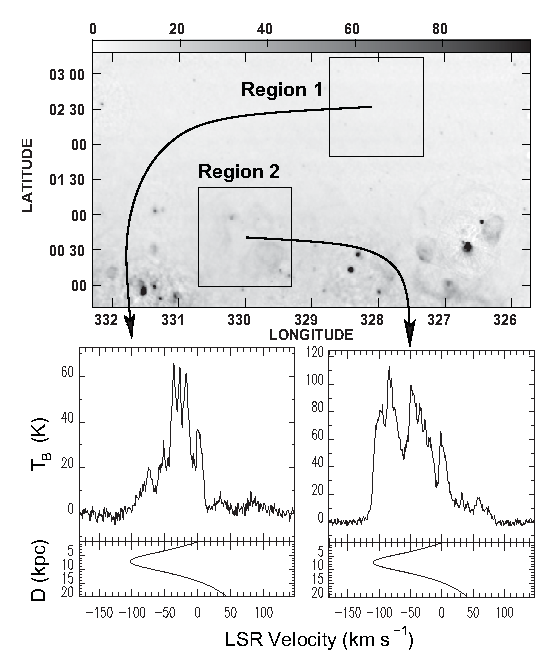
\includegraphics[totalheight=80 mm]{img/Dickey2001_regions.eps}
              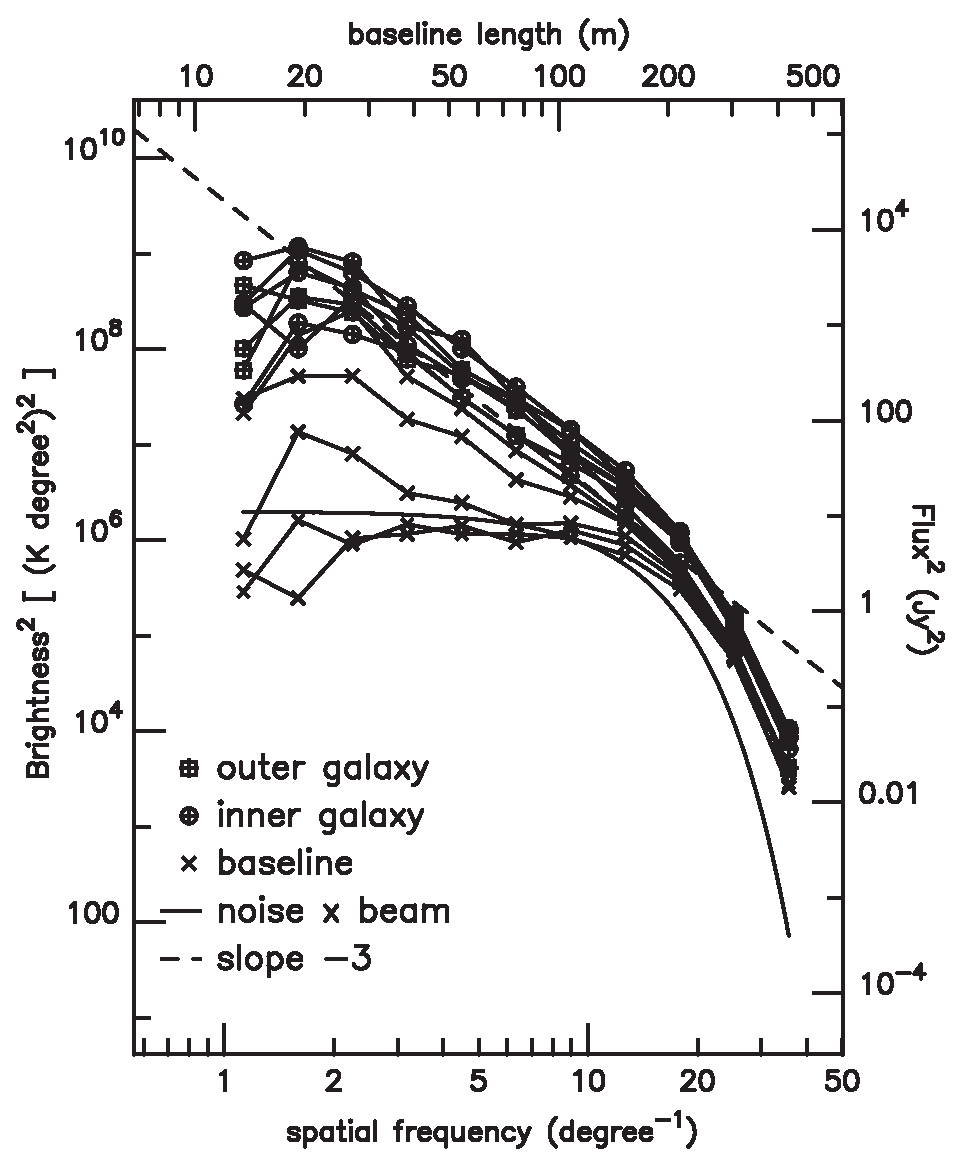
\includegraphics[totalheight=80 mm]{img/Dickey2001_region2.eps}
            \end{figure}   
        \clearpage
        \begin{small}
        Southern Galactic plane H\textsc{i} survey by \cite{2001ApJ...561..264D}.
        \end{small}
            \begin{figure}[hb]
              \centering
              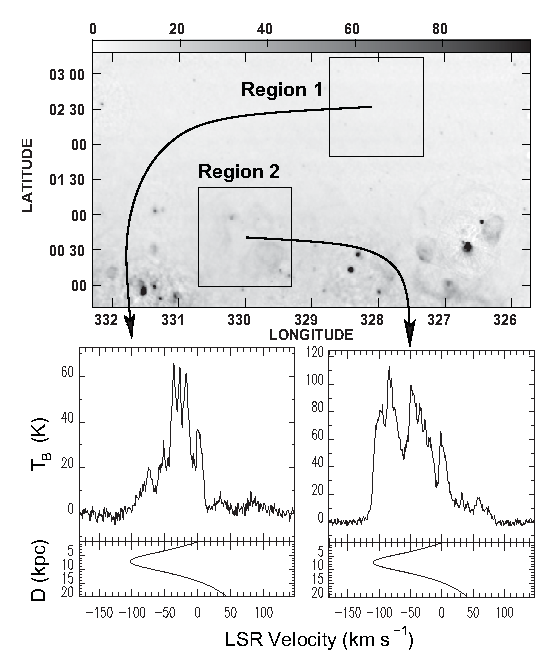
\includegraphics[totalheight=80 mm]{img/Dickey2001_regions.eps}
              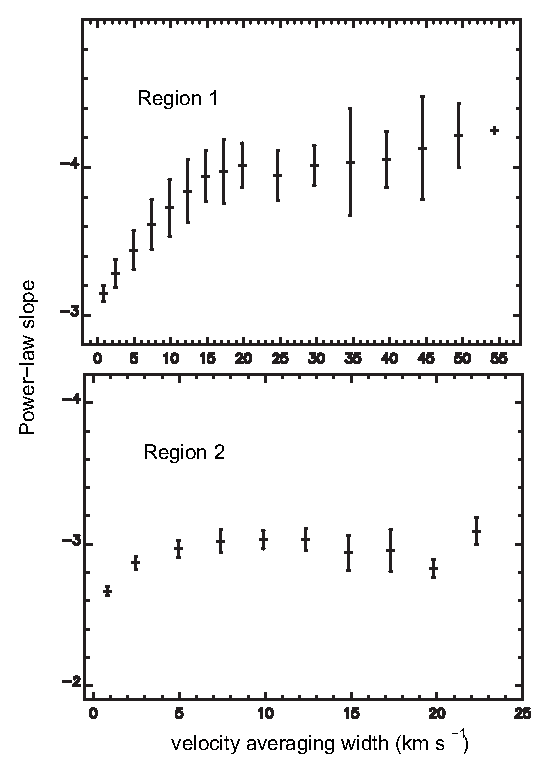
\includegraphics[totalheight=80 mm]{img/Dickey2001_region1+2.eps}
            \end{figure}   
        \clearpage
        \begin{small}
        $P(k)\propto k^{-2.5}$ obtained from IRAS 100 $\mu$m by \cite{1998ApJ...500..525S}.
        \end{small}
            \begin{figure}[hb]
              \centering
              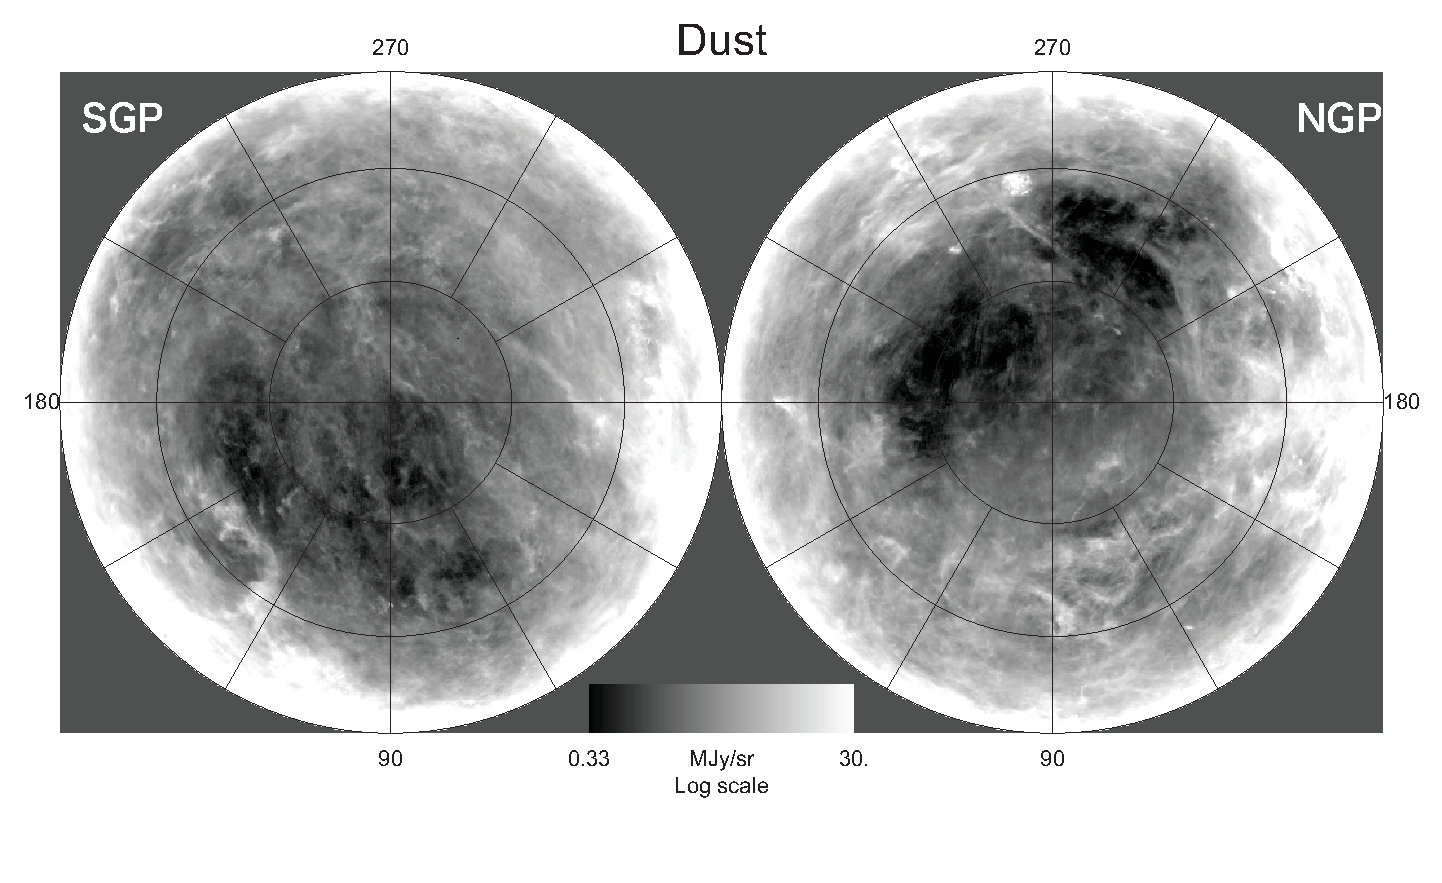
\includegraphics[totalheight=80 mm]{img/Schlege1998_map.eps}
            \end{figure}   
                \clearpage
        \begin{small}
        $P(k)\propto k^{-2.5}$ obtained from IRAS 100 $\mu$m by \cite{1998ApJ...500..525S}.
        \end{small}
            \begin{figure}[hb]
              \centering
              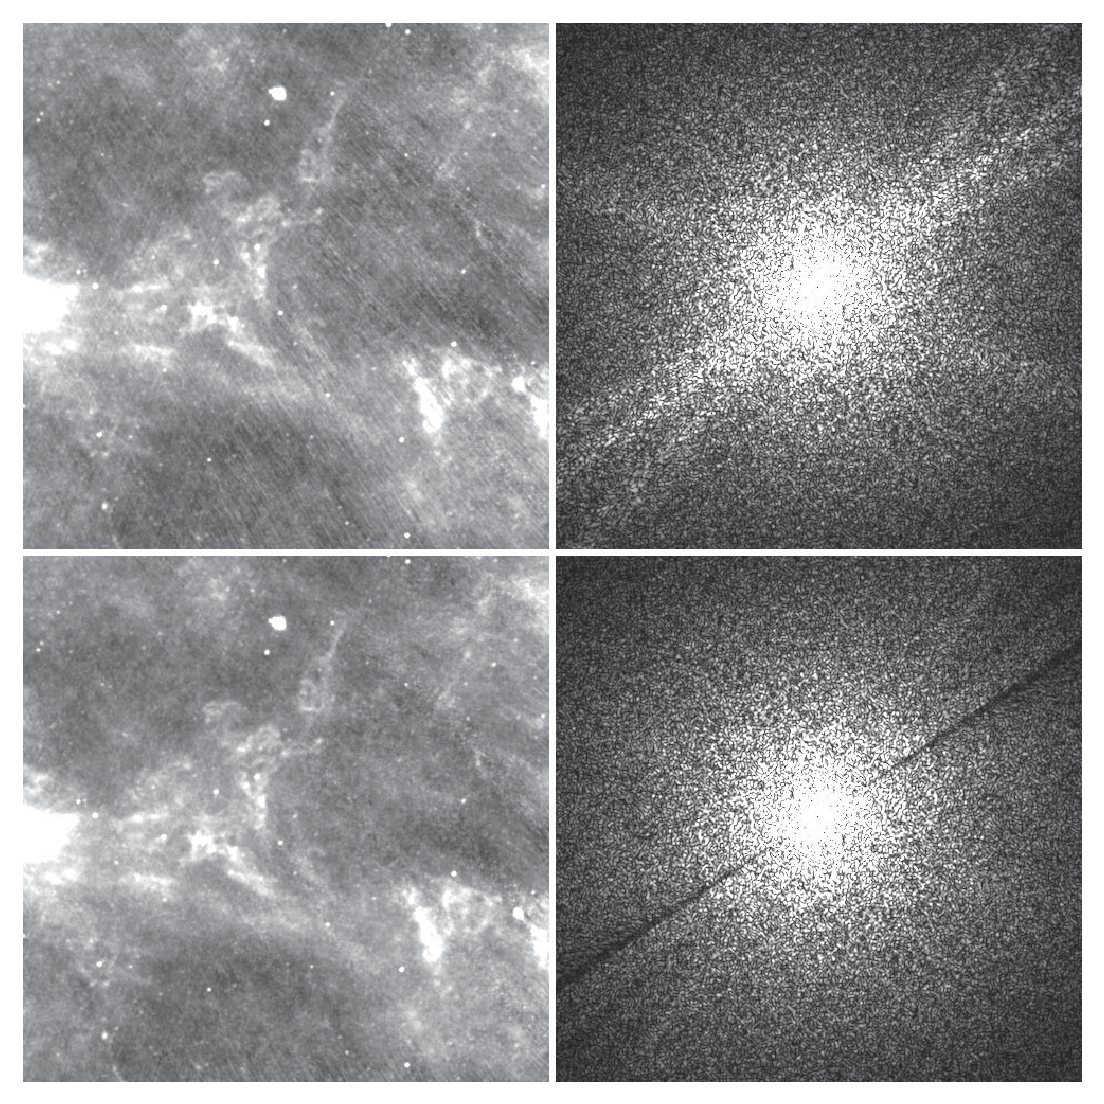
\includegraphics[totalheight=80 mm]{img/Schlege1998_fft.eps}
            \end{figure}   
        \clearpage
        \begin{small}
        $P(k)\propto k^{-2.5}$ obtained from IRAS 100 $\mu$m by \cite{1998ApJ...500..525S}.
        \end{small}
            \begin{figure}[hb]
              \centering
              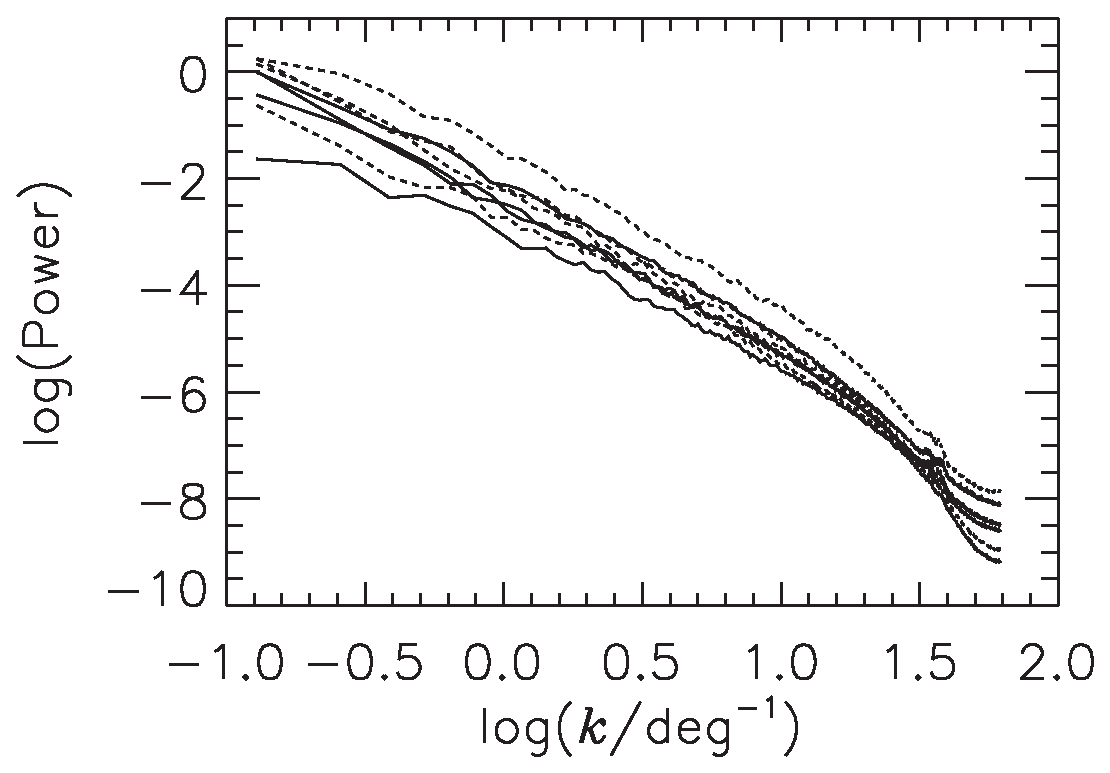
\includegraphics[totalheight=80 mm]{img/Schlege1998_power.eps}
            \end{figure} 
        \clearpage
        \begin{small}
        How well can we resolve it? Figures by \cite{2001A&A...366..636B}.
        \end{small}
            \begin{figure}[hb]
              \centering
              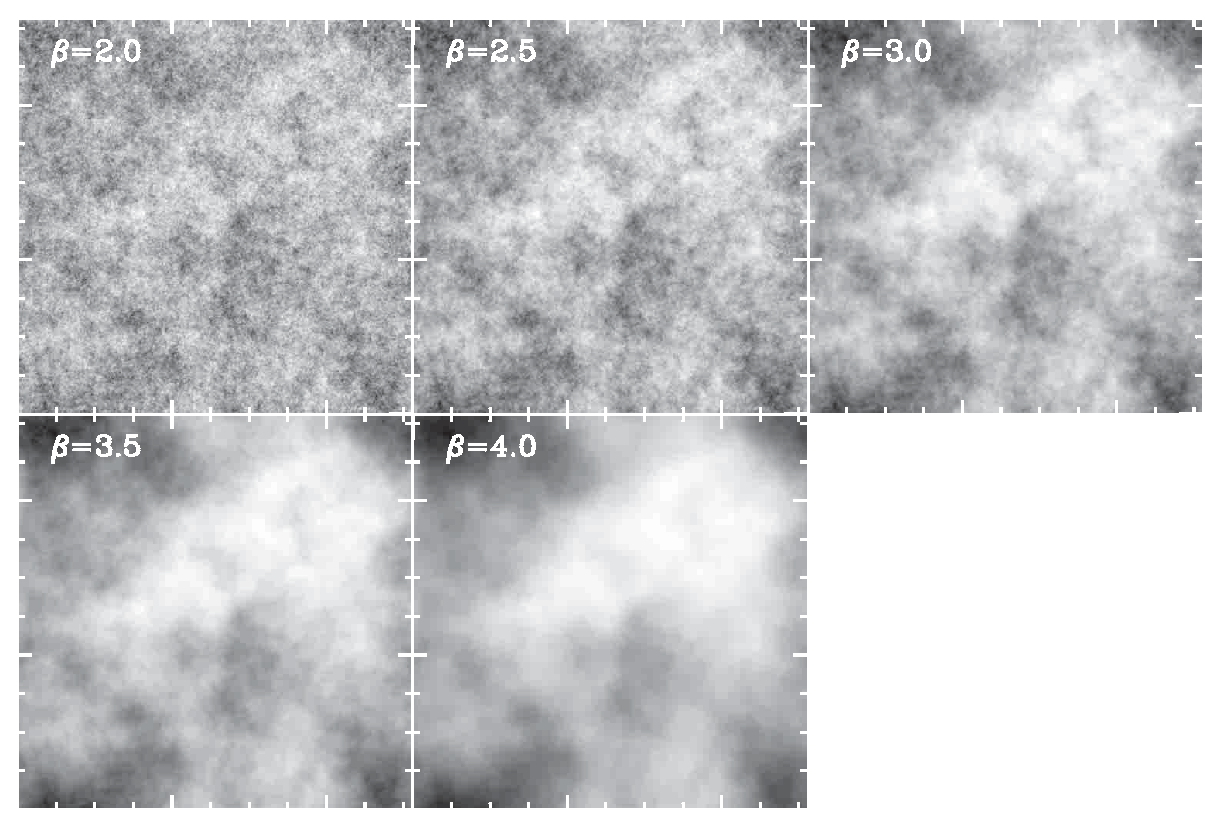
\includegraphics[totalheight=80 mm]{img/2001Bensch.eps}
            \end{figure} 
                \clearpage
        \begin{small}
        \cite{2001A&A...366..636B}.
        \end{small}
            \begin{figure}[hb]
              \centering
              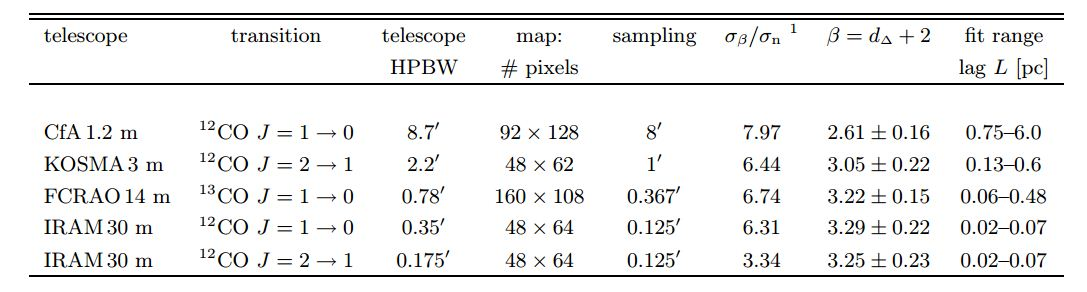
\includegraphics[totalheight=40 mm]{img/Bensch2001_table.JPG}
            \end{figure} 
        \clearpage
        \begin{small}
        Mapping using \coaa, \cobb and \cocc, towards Polaris Flare, by \cite{2001A&A...366..636B}.
        \end{small}
            \begin{figure}[hb]
              \centering
              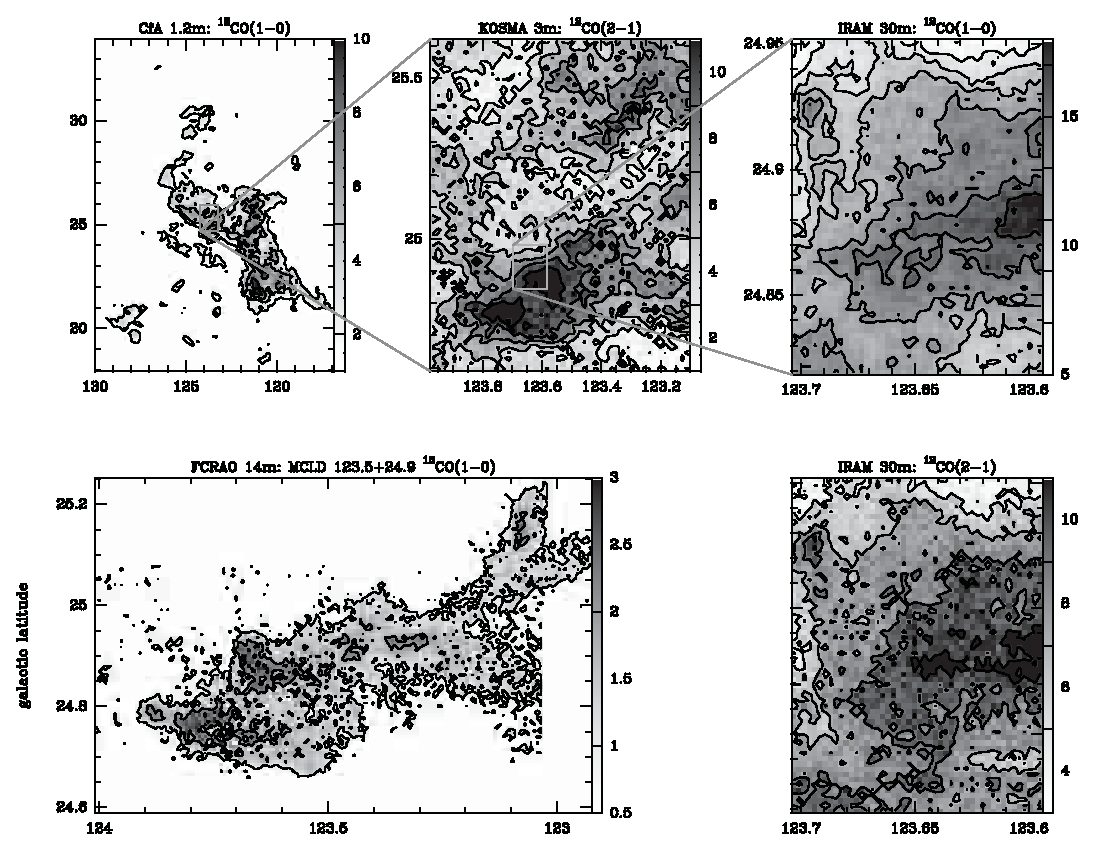
\includegraphics[totalheight=80 mm]{img/Bensch_2001_regionmaps.eps}
            \end{figure} 
        \clearpage
        \begin{small}
        Mapping using \coaa, \cobb and \cocc, towards Polaris Flare, by \cite{2001A&A...366..636B}.
        \end{small}
            \begin{figure}[hb]
              \centering
              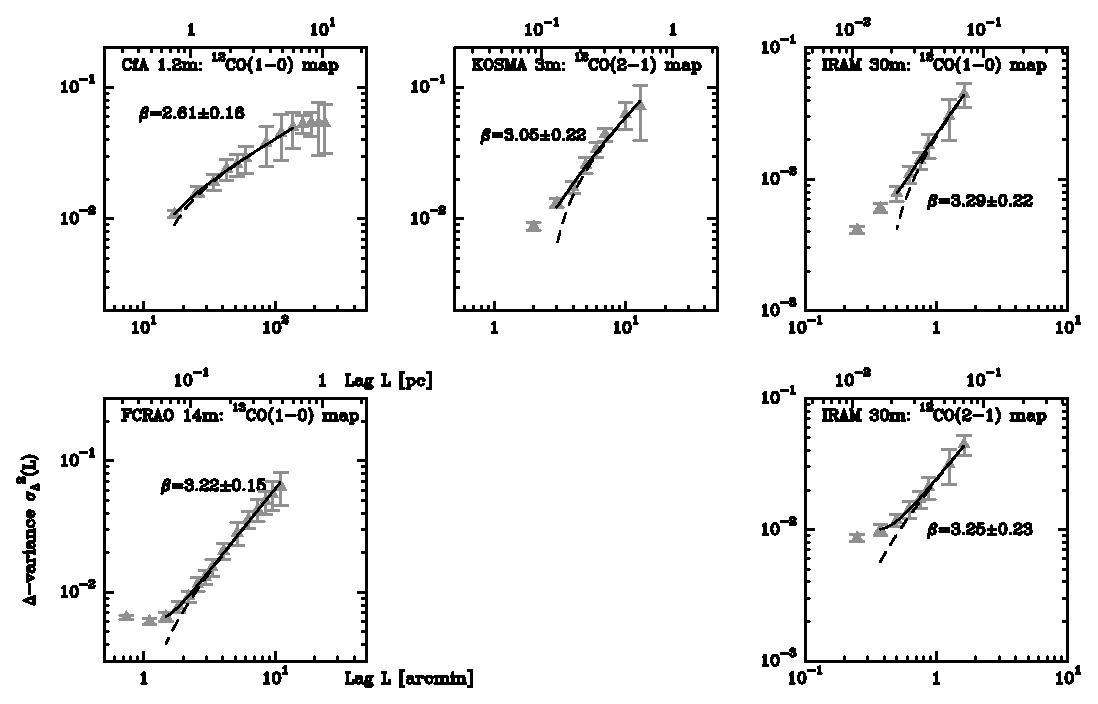
\includegraphics[totalheight=80 mm]{img/Bensch_2001_fivetelescopes.eps}
            \end{figure} 
        \clearpage
        \begin{small}
        Mapping using \coaa, \cobb and \cocc, various regions, by \cite{2001A&A...366..636B}.
        \end{small}
            \begin{figure}[hb]
              \centering
              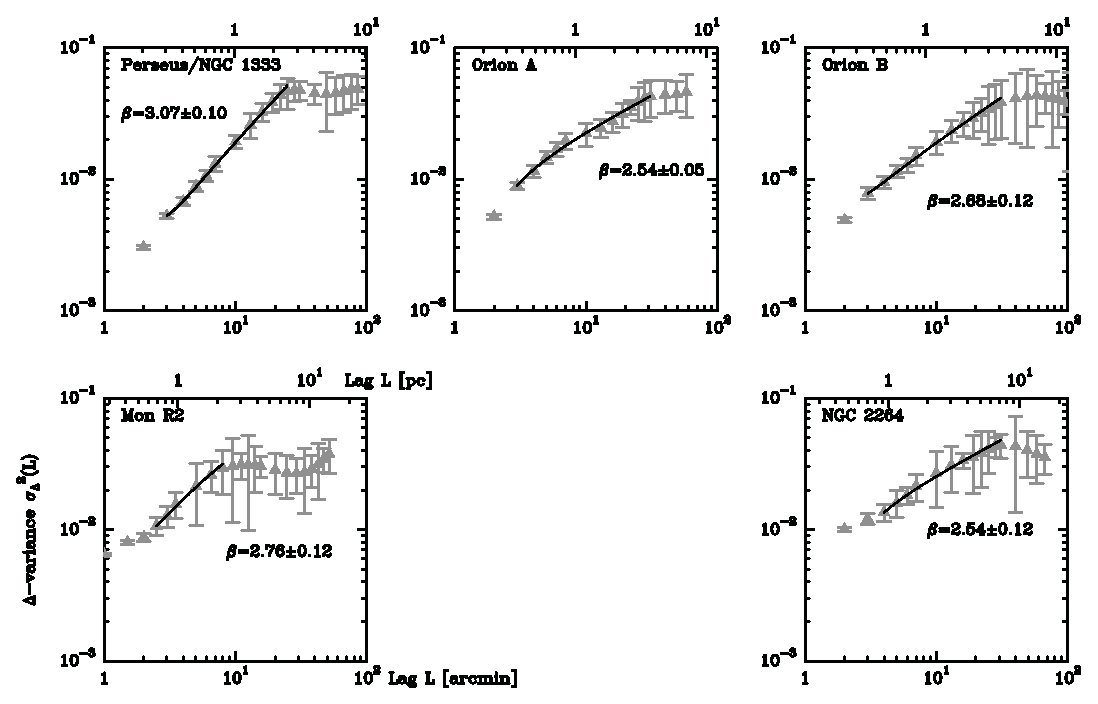
\includegraphics[totalheight=80 mm]{img/Bensch_2001_variousregions.eps}
            \end{figure} 
    % subsection energy_spectrum (end)
% section kolmogorov_s_5_3_theory (end)
\clearpage
\section{PDF Determined by Turbulence} % (fold)
\label{sec:pdf_determined_by_turbulence}
    \begin{small}
    Probability distribution functions (PDFs) of \emph{Herschel} column density maps of Orion B, Aquila, and Polaris, obtained with the \emph{Herschel} Gould Belt survey (HGBS) \citep{2013ApJ...766L..17S}. 
    \end{small}

    Orion B:

    \begin{figure}[hb]
              \centering
              \includegraphics[totalheight=60 mm]{img/Schneider_densityprofile.eps}
    \end{figure} 
\clearpage
    \begin{equation}
        p(\eta)\dd \eta = \frac{1}{\sqrt{2\pi \sigma^2_{\eta}}}e^{-\frac{(\eta-\mu)^2}{2\sigma^2_\eta}} \dd \eta
    \end{equation}
    \begin{figure}[hb]
              \centering
              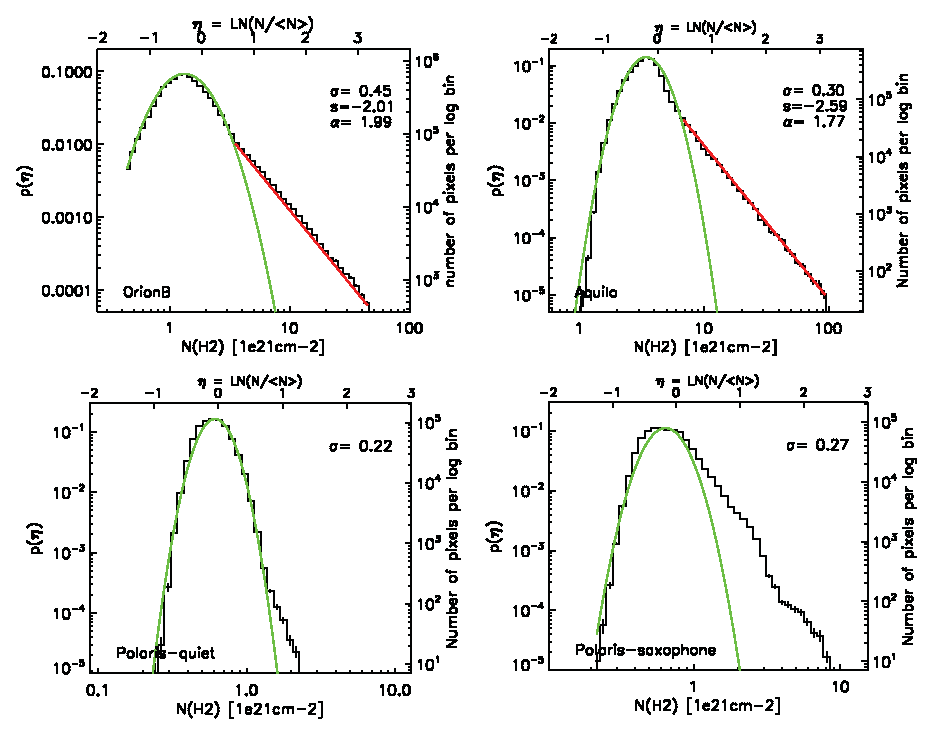
\includegraphics[totalheight=70 mm]{img/Schneider_pdf.eps}
    \end{figure} 
\clearpage

    \begin{figure}[hb]
              \centering
              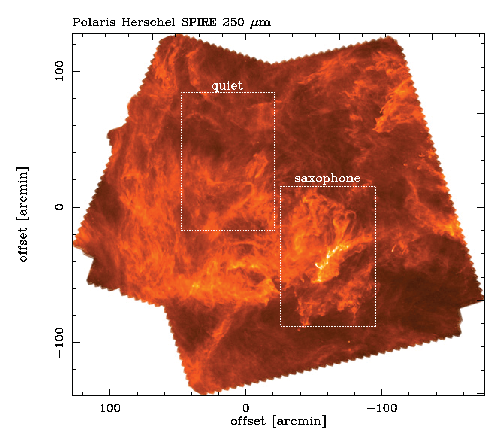
\includegraphics[totalheight=80 mm]{img/Schneider_polaris.eps}
    \end{figure} 

% section pdf_determined_by_turbulence (end)
\clearpage
\section{Simulations of Interstellar Turbulence} % (fold)
\label{sec:simulations_of_interstellar_turbulence}
    \subsection{Scaling Relations} % (fold)
    \label{sub:scaling_relations}
    L: Timescale: 20.2 Myr, different resolutions, power law whose slopes are -0.8 and -5.2.
    R: Timescale: 48 Myr, highest resolutions (4096$^{2}$), power law whose slopes are -0.8 and -1.5. Dashed represent incompressible flow. \cite{2002ApJ...577..197W}
        \begin{figure}[hb]
                  \centering
                  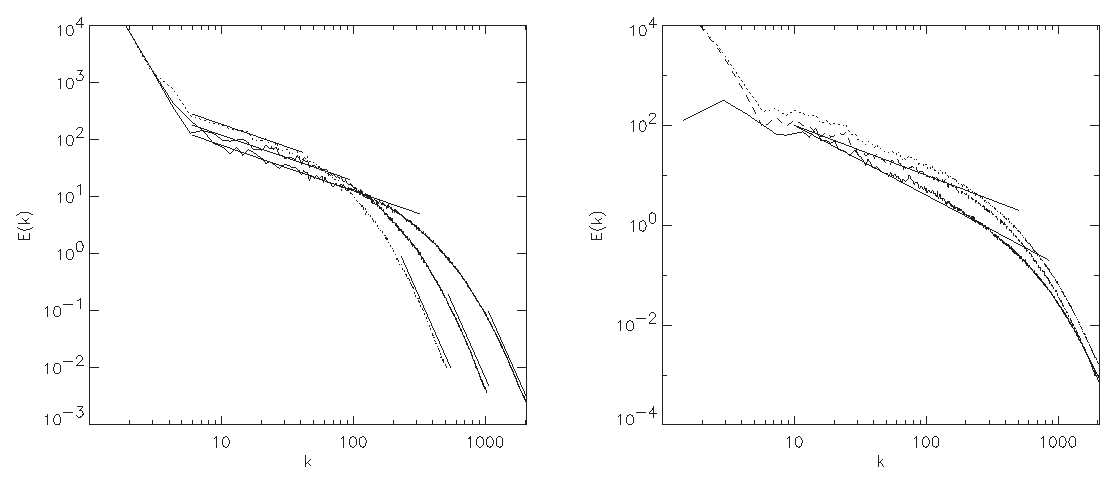
\includegraphics[totalheight=50 mm]{img/Wada.eps}
        \end{figure} 
    \clearpage
    MHD conditions, strong field. \cite{2003ApJ...590..858V}
        \begin{figure}[hb]
                  \centering
                  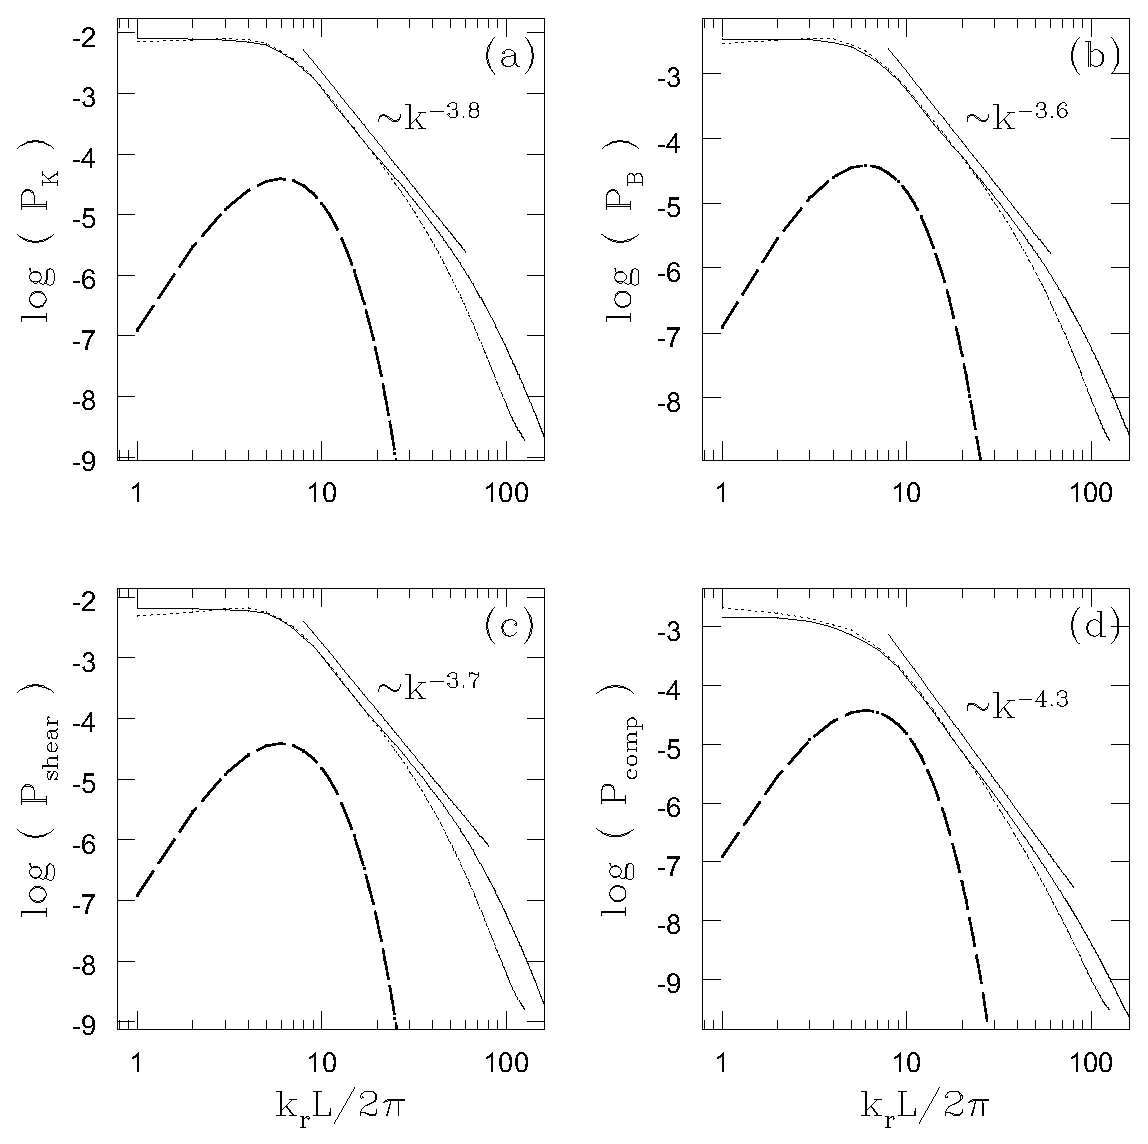
\includegraphics[totalheight=80 mm]{img/Vestuto_strongfield.eps}
        \end{figure} 
    \clearpage
    MHD conditions, weak field. \cite{2003ApJ...590..858V}
        \begin{figure}[hb]
                  \centering
                  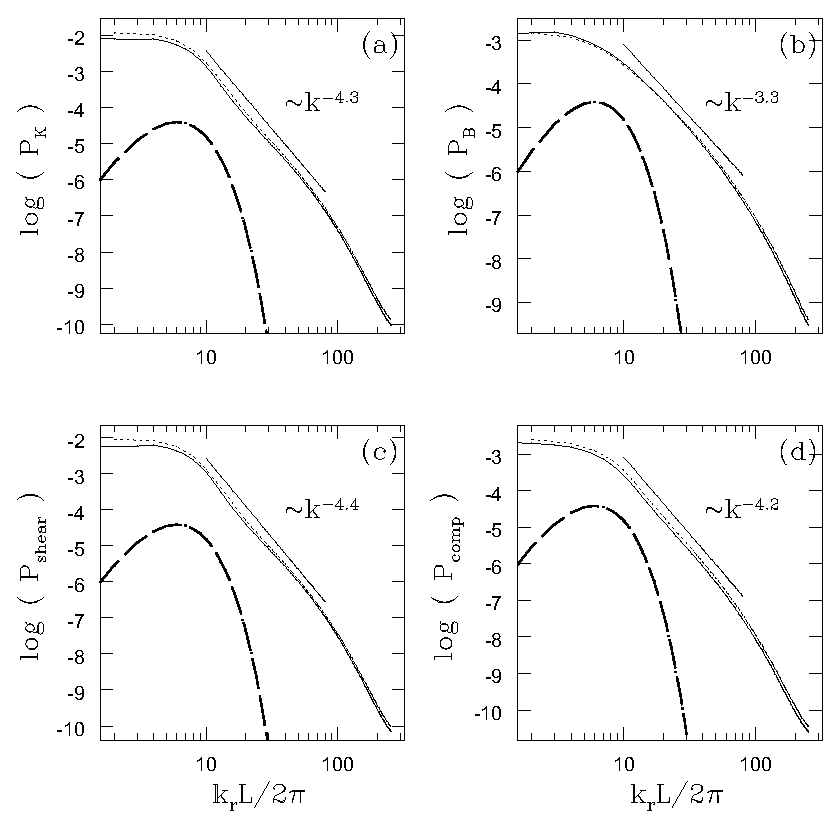
\includegraphics[totalheight=80 mm]{img/Vestuto_weakfield.eps}
        \end{figure} 
    \clearpage
    % subsection scaling_relations (end)
    \subsection{Filaments} % (fold)
    \label{sub:filaments}
    The filaments were identified on the 100 $\mu$m plates of the IRAS Sky Survey Atlas (ISSA), using a computer vision algorithm that is unbiased with respect to source intensity.\cite{2003ApJS..149..365J}
        \begin{figure}[hb]
                  \centering
                  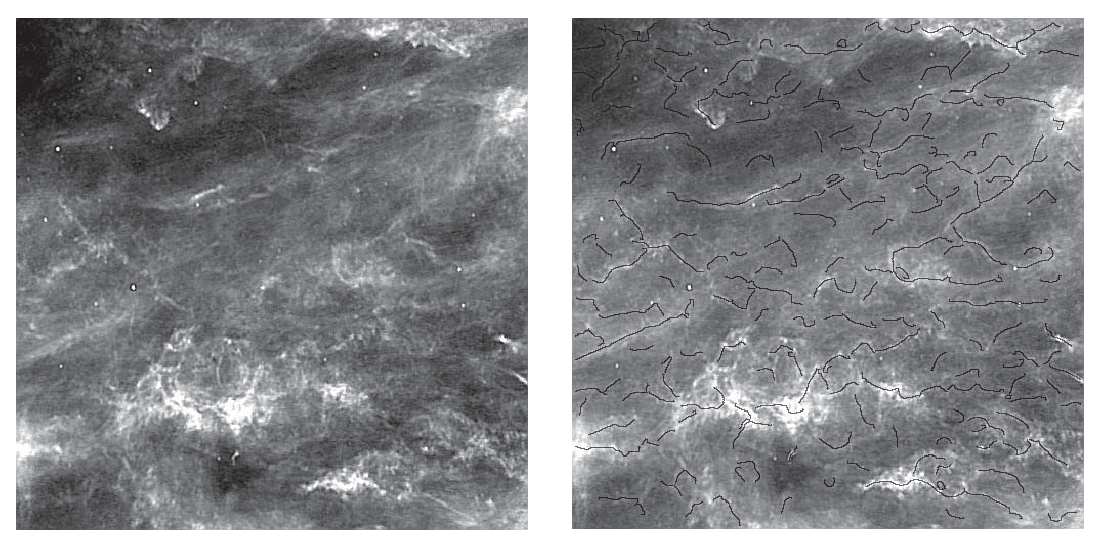
\includegraphics[totalheight=60 mm]{img/Jackson.eps}
        \end{figure} 
    \clearpage
    Criteria for identifying filaments.
    \begin{align}
        I_x &\equiv \frac{\partial I}{\partial x}\\
        I_{xx} &\equiv \frac{\partial^2 I}{\partial x^2}
    \end{align}
    More generally:
    \begin{align}
        I_v &= \hat{\vec{v}}\cdot \nabla \vec{I}\\
        I_{uv} &= \hat{\vec{u}}\cdot \nabla(\hat{\vec{v}}\cdot \nabla \vec{I})
    \end{align}
    \clearpage
    To rotate the coordinate frame to the direction parallel (perpendicular) to the filament, we firstly define an angle:
    \begin{equation}
        \beta  = \frac{1}{2} \tan ^{-1} \frac{2I_{xy}}{I_{xx}-I_{yy}}
    \end{equation}
    Thus:
    \begin{equation}
        \left(\begin{array}{c}
            \partial_p\\
            \partial_q
        \end{array}\right)
        =
        \left(\begin{array}{rr}
            \sin \beta & -\cos \beta\\
            \cos \beta & \sin \beta
        \end{array}\right)
        \left(\begin{array}{c}
            \partial_x\\
            \partial_y
        \end{array}\right)
    \end{equation}
    Basic properties:
    \begin{equation}
        |I_{pp}|>|I_{qq}|,\ I_{pp}<0,\ I_p=0
    \end{equation}
    % subsection filaments (end)
% section simulations_of_interstellar_turbulence (end)
\clearpage
\section{Summary} % (fold)
\label{sec:summary}
\clearpage
% section summary (end)
\centering
\vspace{50 mm}

\begin{LARGE}{\textbf{Questions?}}\end{LARGE}
\clearpage
\bibliography{Turbulence}
\end{document}
